\documentclass[a4paper, 12pt]{article}
\usepackage[T2A]{fontenc} 
\usepackage[utf8]{inputenc}
\usepackage[english,russian]{babel} 


\usepackage{amsmath,amsfonts,amssymb,amsthm,mathtools}

\usepackage[left=2cm,right=2cm,top=2cm,bottom=2cm,bindingoffset=0cm]{geometry}

\usepackage{graphicx}

\newtheorem*{theorem}{Теорема}
\newtheorem*{corollary}{Следствие}
\newenvironment{Proof}
{\par\noindent{$\blacklozenge$}}
{\hfill$\scriptstyle\boxtimes$}

\usepackage[normalem]{ulem}
\usepackage[unicode]{hyperref}

\newcommand{\R}{\operatorname{R}}
\renewcommand{\Re}{\operatorname{Re}}
\renewcommand{\Im}{\operatorname{Im}}

\title{\vspace{6.5cm}\textbf{\Huge{Алгебра и Теория чисел}}\\Конспект по 1 семестру 
специальности «прикладная информатика»\\(лектор Г. В. Матвеев)}
\date{}
\begin{document}
\maketitle
\newpage
\tableofcontents{}
\newpage

\section{Операции над комплексными числами}
Множество комплексных чисел имеет вид:
$$C=\{a+bi \: |a,b \in \R \}$$
где $i$ - мнимая единица.\\\\
$\bullet$ По определению $i^2=-1$\\\\
Общий вид комлексного числа имеет вид:
$$z = a + bi$$
$a = \Re z$ - \textbf{вещественная} часть числа $z$\\
$b = \Im z$ - \textbf{мнимая} часть числа $z$.\\\\
\textit{\textbf{Операции над комплексными числами:}}\\
\begin{enumerate}
    \item \textit{Сложение и вычитание комплексных чисел}
    $$(a+bi) \pm (c+di) = (a \pm c) + (b \pm d)i$$
    \item \textit{Сравнение комплексных чисел}
    $$a+bi = c+di \Leftrightarrow \begin{cases} a = c,\\ b = d. \end{cases}$$
    \item \textit{Нулевое комплексное число}
    $$a + bi = 0 \Leftrightarrow \begin{cases} a = 0,\\ b = 0. \end{cases}$$
    \item \textit{Умножение комплексных чисел}
    $$(a+bi)(c+di)=(ac-bd)+(ad+bc)i$$
    \item \textit{Деление комплексных чисел}
    $$\frac{a+bi}{c+di} = \frac {(a+bi)(c-di)}{(c+di)(c-di)} = \frac {ac+bd}{c^2+d^2}+\frac{bc-ad}{c^2+d^2}i$$
\end{enumerate}
\textit{\textbf{Свойства сложения и умножения:}}
\begin{enumerate}
    \item \textit{Коммутативность}
    $$z_1 + z_2 = z_2 + z_1$$
    $$z_1z_2=z_2z_1$$
    Коммутативность комплексных чисел вытекает из коммутативности вещественных.
    \item \textit{Ассоциативность}
    $$z_1 + (z_2 + z_3) = (z_1 + z_2) + z_3$$
    $$z_1(z_2z_3)=(z_1z_1)z_3$$
    \item \textit{Существование противоположного числа}
    $$\forall z, \exists -z, \: z+(-z)=0$$
    \item \textit{Дистрибутивность}
    $$z_1(z_2+z_3)=z_1z_2+z_1z_3$$
\end{enumerate}
\subsection{Геометрическая интерпретация комплексных чисел}
$\bullet$ $\overline{z}=a-bi$ - сопряженное число числа $z=a+bi$\\
\begin{figure}[ht]
\centering
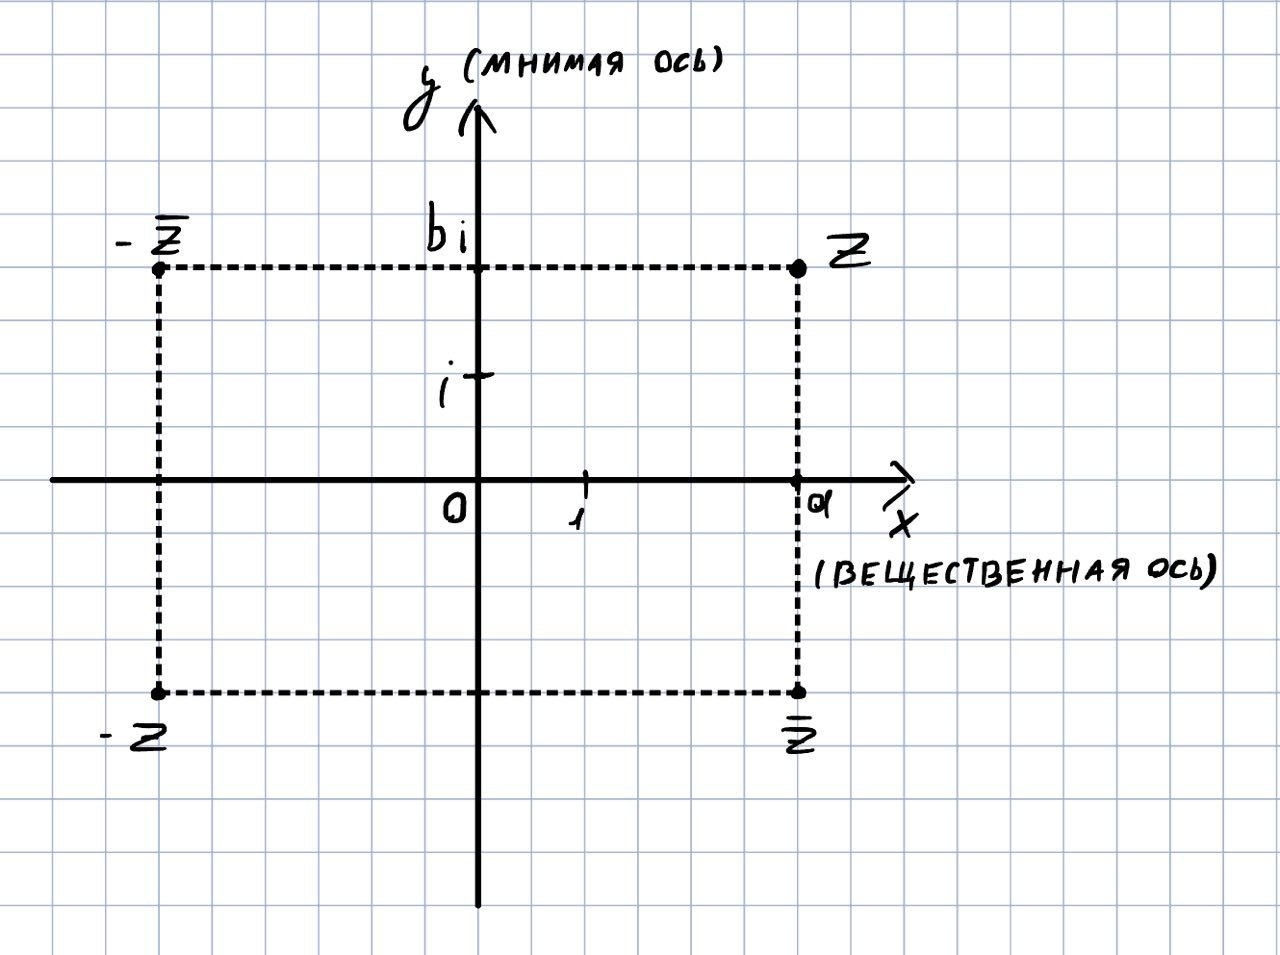
\includegraphics[width=0.5\linewidth]{pict1.jpg}
\caption{Комплексные числа на плоскости}
\label{fig:reg}
\end{figure}\\
\textit{\textbf{Свойства сопряженного числа:}}
\begin{enumerate}
    \item $\overline{\overline{z}}=z$
    \begin{Proof}
        $\overline{\overline{a+bi}} = \overline{a-bi} = a+bi = z$
    \end{Proof}
    \item $\overline{z_1+z_2} = \overline{z_1}+\overline{z_2}$
    \begin{Proof}
        $\overline{z_1+z_2}=\overline{a+bi+c+di}=\overline{(a+c)+(b+d)i} = (a+c)-(b+d)i$\\
        $\overline{z_1}+\overline{z_2}=a-bi+c-di=(a+c)-(b+d)i=\overline{z_1+z_2}$
    \end{Proof}
    \item $\overline{z_1 \cdot z_2}=\overline{z_1}\cdot\overline{z_2}$
    \begin{Proof}
        $\overline{z_1}\cdot\overline{z_2}=(a-bi)(c-di)=(ac-bd)-(ad+bc)i$\\
        $z_1\cdot z_2=(a+bi)(c+di)=(ac-bd)+(ad+bc)i$\\
        $\overline{z_1\cdot z_2} = (ac-bd)-(ad+bc)i = \overline{z_1}\cdot\overline{z_2}$
    \end{Proof}
    \item $\overline{(\frac{z_1}{z_2})} = \frac{\overline{z_1}}{\overline{z_2}}$
    \begin{Proof}
        $\frac{z_1}{z_2}=\frac{a+bi}{c+di}\cdot \frac{c-di}{c-di}=\frac{ac+bd}{c^2+d^2}+\frac{bc-ad}{c^2+d^2}$\\
        $\overline{(\frac{z_1}{z_2})}=\frac{ac+bd}{c^2+d^2}+\frac{ad-bc}{c^2+d^2}i$\\
        $\frac{\overline{z_1}}{\overline{z_2}}=\frac{a-bi}{c-di} \cdot \frac{c+di}{c+di} = \frac{ac+bd}{c^2+d^2}+\frac{ad-bc}{c^2+d^2}i = \overline{(\frac{z_1}{z_2})}$
    \end{Proof}
    \item $z\cdot \overline{z} = (a+bi)(a-bi)=a^2+b^2$
\end{enumerate}
\begin{center}
    \textbf{Модуль комплексного числа}
\end{center}
$$|z|=\sqrt{a^2+b^2}=\sqrt{z\cdot\overline{z}}, \quad |z| \in \R$$
\textit{\textbf{Свойства модуля:}}
\begin{enumerate}
    \item $|z_1\cdot z_2|=|z_1|\cdot |z_2|$
    \item $|z_1+z_2| \leq |z_1| + |z_2|$
    \item $z=0 \Leftrightarrow |z|=0$
\end{enumerate}

\end{document}
